\documentclass[12pt, a2paper, landscape]{tikzposter}
\usepackage[utf8]{inputenc}
\usepackage{amsmath}
\usepackage{amsthm}
\usepackage{color}
\usepackage{xcolor}
\usepackage{dirtytalk}
\UseRawInputEncoding
\usepackage{graphicx}
\usepackage{caption}
\usepackage{subcaption}
\usepackage{mathtools}
\usepackage[thinc]{esdiff}
\usepackage{tocbibind}
\usepackage{parskip}
\usepackage[ruled,vlined]{algorithm2e}
\newtheorem{theorem}{Theorem}
\newtheorem{definition}{Definition}
\graphicspath{ {./images/} }


\title{Decision Trees}
\author{Pattanin (Mill) Luangamornlert, Supervised by Peter Craig and Louis Aslett}
\institute{Durham University}
\usetheme{Rays}
\usecolorstyle{Australia}
\usetitlestyle{VerticalShading}
\useblockstyle{Basic}


\begin{document}
\maketitle

 
\begin{columns}
 \column{0.25}
 \block{What are Decision Trees}{
 Decision Trees are a method of supervised Machine Learning.
 Invented in 1984 \cite{BreimanDT}, 
 CART is the most famous and popular method for Decision Trees and relies on checking impurities in the splitting of data in feature selection.
 \bigskip\\
 For a dataset, we aim to split the data $\{x_{i}, y_{i}\}_{i=1}^{n}$ into $R_m$ regions, $m = [1, \dots, M]$.\\
 For each split, we calculate one of the two metrics below, depending on whether it is a classification or regression problem, to decide where to split the data at each partition.
 \begin{tikzfigure}
    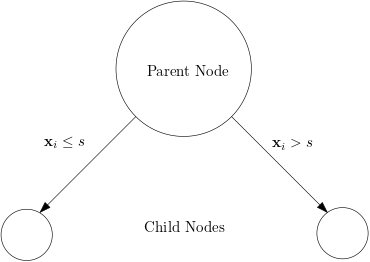
\includegraphics[width=0.125\textwidth]{ipefile/simpledecisionsplit.png}
    \label{fig:dt1}
 \end{tikzfigure}
 }

 
 \block{Classification - Gini Impurity}{
 To select splitting points, CART uses Gini Impurity in selecting features.\\
 Gini Impurity is defined as follows:
 \begin{equation}
    I_G (p) = I_G (p_1, \dots, p_M) = \sum_{i=1}^{M} p_i(1-p_i)
 \end{equation}
 From here we apply this equation to all variables and select the one which provides the highest impurity, i.e. $\max$ $I_G (p)$, as the splitting point.
 }
 \column{0.25}
 \block{Regression - RSS}{
 Suppose we have a space $R$ and we have $M$ partitions, we first partition the space into $M$ regions $R_1, \dots, R_M$.\\
 To construct the regions, we try to find regions which minimize RSS, where we have $\hat{y}_{R_m}$ as the mean response for each region:
 \begin{equation}
    RSS = \sum_{m=1}^{M} \sum_{i \in R_m} (y_i - \hat{y}_{R_m})^2
 \end{equation}
 From here we apply this equation to all variables and select the one which provides the smallest error, i.e. $\min$ RSS, as the splitting point.
 This equation is:
 \begin{equation}
    \min \sum_{x_i \in R_1} (y_i - \hat{y}_{R_1})^2  +  \sum_{x_i \in R_2} (y_i - \hat{y}_{R_2})^2
 \end{equation}
 }
 
 \block{Meta-Algorithm for Trees}{
 Here is the algorithm for decision trees:
 \begin{enumerate}
     \item Use recursive splitting at all points into regions $R_1, R_2$ such that for a splitting value $s$, we have that for each value $x_i$, $i \in [1, \dots, n]$:
     \begin{enumerate}
         \item $R_1 = x_i \leq s$
         \item $R_2 = x_i > s$
     \end{enumerate}
     and classify each prediction in region based on the mean/modal value in each region
     
     \item Calculate the metric value for each region
     
     \item Compare metric values to find the most optimal splitting point
     
     \item Repeat until stopping criterion met
 \end{enumerate}

 }
 
 
 \column{0.25}

 
 \block{Pruning}{
    To achieve interpretability, we would prefer smaller trees. However, growing small trees would hide useful splits hidden under weak splits. Therefore a more optimal approach would be to grow the tree and then cut back to a more optimal size.\\
    The idea of pruning is to minimise the cost-complexity criterion $C_{\alpha} (T)$:
    \begin{equation}
        C_{\alpha} (T) = R(T) + \alpha \left|T\right|
    \end{equation}
    Where $R(T)$ is the learning error, $\left|T\right|$ the number of terminal nodes in tree $T$, and $\alpha$ the regularization parameter. We find that $\alpha$ can be obtained from:
    \[ \alpha = \frac{R(t)-R(T_t)}{|T_t| - 1} \]
    The algorithm for this is as such:
    \begin{enumerate}
        \item Initialization - Let $T^1$ be the tree obtained with $\alpha^1 = 0$ by minimizing $R(T)$
    
        \item Select $t \in T^1$ which minimizes
        \[ g_1 (t) = \frac{R(t)-R(T_t^1)}{|T_t^1| - 1} \]
    
        \item Let $t_1$ be this node and let $\alpha^2 = g_1 (t_1)$ which results in $T^2 = T^1 - T_{t_1}^1$
    
        \item Repeat the process $i$ times until at cost $k$
    \end{enumerate}
    After pruning, we have found an optimal tree which provides the highest accuracy score.
 }
 
 \block{}{
 \bibliography{reference}
 }
 
 \column{0.25}
 \block{Salary Example}{
 Here is an example using baseball data. We use the \texttt{rpart} \cite{rpart} algorithm to perform this action.
 }
 
 

 
\end{columns}



\bibliographystyle{siam}


\end{document}